% samplepaper.tex: springer.com
% modificato da MM 06/05/2018
%

\documentclass[runningheads]{llncs}
\usepackage[italian]{babel}
\usepackage{csquotes}
\usepackage{graphicx}
\usepackage{subfigure}
\usepackage{listings}
\usepackage{threeparttable}
% Used for displaying a sample figure. If possible, figure files
% should be included in EPS format.  If you use the hyperref package,
% please uncomment the following line to display URLs in blue roman
% font according to Springer's eBook style:
% \renewcommand\UrlFont{\color{blue}\rmfamily}
\begin{document}
%
\title{Sistema IR per collezione di articoli medici utilizzando diversi insiemi di stopword}
%
\titlerunning{Sistema IR per collezione OHSUMED}
% If the paper title is too long for the running head, you can set
% an abbreviated paper title here
%
\author{%
  Alessandro Stefani\inst{1} \and
  Caterina Buranelli\inst{2} \and
  Cristi Gutu\inst{3}}
%
\authorrunning{Alessandro Stefani, Caterina Buranelli, Cristi Gutu}
% First names are abbreviated in the running head.  If there are more
% than two authors, 'et al.' is used.
%
\institute{Corso di laurea in Statistica per le tecnologie e le scienze,
  matricola 1148387 \email{alessandro.stefani.6@studenti.unipd.it} \and Corso di laurea in Statistica per le tecnologie e le scienze,
    matricola 1163443 \email{caterina.buranelli@studenti.unipd.it} \and Corso di laurea in Statistica per le tecnologie e le scienze,
      matricola 1147351 \email{gheorghecristi.gutu@studenti.unipd.it}
  }
%
\maketitle

%
\begin{abstract}
Questo progetto tratta la realizzazione attraverso il pacchetto \emph{Whoosh}, di un motore di ricerca
volto al reperimento di documenti della collezione sperimentale \emph{OHSUMED} indicizzata opportunamente.
Si \`e affrontato il problema della valutazione del sistema di ricerca studiando l'effetto dell'esclusione
di diversi insiemi di stopword. Nella relazione verr\`a evidenziato come l'uso delle stopword migliori l'efficacia
del sistema IR.
Il progetto \`e anche corredato di un webserver che permette all'utente di interrogare il motore di ricerca
in forma interattiva, attraverso un browser a scelta.
 \keywords{{\it
      Information Retrieval  \and IR \and statistica \and reperimento \and indicizzazione \and Whoosh \and Python \and webserver \and web \and interrogazione web  \and stopword}}
\end{abstract}

\section{Introduzione}
\label{sec:introduzione}

Lo scopo finale di un Sistema di Information Retrieval (IRS) \`e quello di reperire documenti
 rilevanti relativi a una certa esigenza informativa\footnote{insieme delle circostanze in cui una
 persona ha un problema da risolvere o un compito da svolgere richiede informazioni
 importanti, utili o necessarie per la risoluzione del problema o lo svolgimento del compito.};
  dunque i documenti sono il primo input del sistema, mentre il secondo \`e
  costituito dalle interrogazioni; i documenti devono essere
  indicizzati e nell'indice creato si andr\`a a effettuare la ricerca per reperire documenti rilevanti\footnote{la rilevanza \`e la propriet\`a che rende l'informazione importante, utile o necessaria a soddisfare l'esigenza informativa dell'utente.}. 
  
  Questa seconda parte \`e detta reperimento e non si occupa solo di ricercare tra i documenti, ma anche di riordinare secondo un certo ordine di rilevanza. 
  
  Ci\`o che descrive i documenti e ci\`o che descrive le interrogazioni deve essere confrontabile, infatti nei programmi di indicizzazione e di reperimento si usa uno schema, che si deve tenere in considerazione per entrambi i casi.

  
L'indicizzazione \`e un trade-off tra il  miglioramento della rappresentazione del
contenuto informativo dei documenti (efficacia) e la gestione degli indici (efficienza), in questa relazione si tratter\`a il problema dell'efficacia.
Esistono diversi modi per risolvere questo problema; nel nostro caso 
ci concentriamo sull'utilizzo di stopword.


\vspace{\baselineskip}

Il resto della relazione \`e organizzato come segue. Nella sezione 2, si descrivono
alcuni dei metodi standard, i pi\`u didattici, su cui si basano gli esperimenti.
La sezione 3, presenta l'interfaccia web e le sue modalit\`a di utilizzo.
Nella sezione 4, sono riportati gli esperimenti fatti ed i risultati ottenuti,
commentati e sotto forma di tabelle esplicative. Infine, nella sezione 5,
si traggono delle brevi conclusioni.



\section{Base di partenza}
\label{sec:base-di-partenza}
Un sistema IR si pu\`o basare su vari modelli e metodi di rappresentazione delle informazioni e di reperimento.
Come gi\`a detto, in questa sezione si presenteranno quelli scelti per implementare il motore di ricerca utilizzato negli esperimenti.

\subsection{Indicizzazione}
L'indice creato da whoosh rappresenta la collezione utilizzando un cos\`i detto \emph{inverted index}\cite{WBC_ii} ovvero, una "matrice" in cui si associa ad ogni termine
una lista dei dati rilevanti corrispondenti.

I dati rilevanti possono essere, per esempio, i documenti in cui sono presenti i termini, con le rispettive frequenze.
Ogni elemento della lista \`e detto \emph{posting} e la parte del \emph{posting} che fa riferimento ad uno specifico documento
\`e detta \emph{pointer}.

\vspace{\baselineskip}

In qesto progetto si tratta in particolare dell'eliminazione delle \emph{stopword}\cite{WBC_stopword}.

Questa \`e una procedura di elaborazione del testo, se utilizzata si deve fare sia sui documenti da indicizzare 
che eventualmente sulle query inviate al motore di ricerca.

Le stopword sono parole che non portano informazione significativa da sole e quindi non aiutano a capire se un documento \`e rilevante o meno.
Inoltre, solitamente si tratta di parole molto comuni nella collezione che quindi risultano in un costo rilevante dal punto di vista dello spazio di memoria occupato.

Parole che di solito si identificano come stopword nella lingua inglese sono per esempio: "the", "a", "an", "that" o "those".

Oltre a queste parole, che non hanno significato a se stante, si possono identificare anche stopword a seconda del contesto. 
Con questo si intende che delle parole possono diventare stopword in certi contesti anche se in altri non lo sono, ad esempio nel manuale di
MySQL parole come "mysql" e "table" risultano utilizzate cos\`i di frequente che non aiutano nella ricerca di un particolare argomento.

La costruzione di un insieme di stopword deve essere fatta con cautela, infatti, la rimozione di troppe parole pu\`o peggiorare l'efficacia del motore di ricerca;
per esempio alcune query valide potrebbero non dare alcun risultato.

\begin{figure}%
    \centering
    {{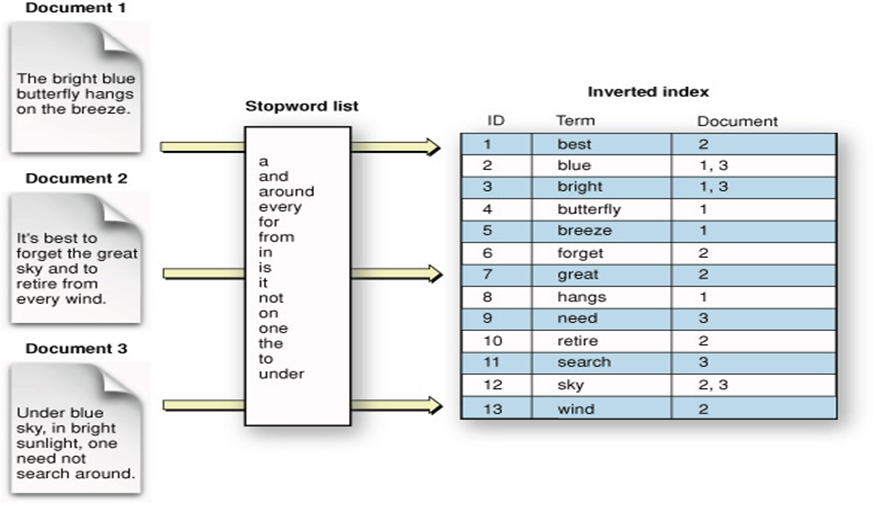
\includegraphics[width=0.8\linewidth]{inverted_index} }}%
    \caption{\emph{Inverted index} e eliminazione delle \emph{stopword}, rappresentati in modo schematico.}%
\end{figure}

\subsection{Reperimento}
Come modello di reperimento si \`e utilizzato il modello probabilistico, paradigma dominante nell'implementazione di sistemi IR.

Questo modello si basa sul Probability Ranking Principle(PRP)\cite{PRP} ovvero:

\blockquote{"Se un Sistema IR risponde a ciascuna interrogazione con una lista di documenti ordinati in
modo non crescente per probabilit\`a di rilevanza all'esigenza informativa dell'utente che ha espresso l'interrogazione,
e posto che le probabilit\`a siano state stimate nel modo migliore possibile sulla base dei dati a disposizione, allora
l'efficacia complessiva del sistema \`e la maggiore possibile sulla base di quei dati."}

In questo modello i documenti sono rappresentati come vettori in cui ogni elemento, relativo ad un termine, assume valore 1 o 0 
a seconda che il termine corrispondente sia presente nel documento o meno.
Inoltre si fa l'assunzione che la presenza di un termine sia indipendente dalla presenza degli altri termini.
Per questo si parla anche di \emph{binary independence model}.

Nel contesto del modello probabilistico, lo schema di pesatura comunemente utilizzato nella funzione che assegna l'ordine ai documenti a seconda del grado di rilevanza \`e il cosiddetto BM25\cite{WBC} (Best Matching 25).

\vspace{1in}

La formula della funzione di scoring per il BM25 \`e:

\begin{figure}
  \centering
  \scalebox{1.5}{$\sum_{i\in Q}[log(\frac{(r_{i}+0.5)/(R-r_{i}+0.5)}{(n_{i}-r_{i}+0.5)/(N-n_{i}-R+r_{i}+0.5)})\cdot \frac{(k_{1}+1)f_{i}}{K+f_{i}}\cdot\frac{(k_{2}+1)qf_{i}}{k_{2}+qf_{i}}]$}
  \end{figure}

Sommatoria su tutti i termini contenuti nella query Q; dove $r_{i}$ \`e il numero di documenti rilevanti contenenti il termine \emph{i}, $n_{i}$ \`e il numero di documenti contenenti il termine \emph{i}, N \`e il numero totale di documenti nella collezione R \`e il numero di documenti rilevanti per la query, $f_{i}$ \`e la frequenza del termine \emph{i} nel documento, $qf_{i}$ \`e la frequenza del termine \emph{i} nella query e $k_{1}$ , $k_{2}$, e K sono parametri i cui valori sono assegnati empiricamente.

Si ha inoltre la condizione che $r_{i}$ e R sono posti a 0 nel caso non ci sia informazione rilevante, i termini 0.5 e 1 servono per evitare complicazioni in questi casi.
\vspace{\baselineskip}



Nella prima parte:
\begin{figure}
\vspace{-10mm}
  \centering
\scalebox{1.5}{$log(\frac{(r_{i}+0.5)/(R-r_{i}+0.5)}{(n_{i}-r_{i}+0.5)/(N-n_{i}-R+r_{i}+0.5)})$},
\vspace{-10mm}
  \end{figure} 
  
il numeratore \`e il rapporto tra il numero di documenti rilevanti in cui il termine \emph{i} appare ed il numero di documenti rilevanti in cui non appare.
In pratica si tratta di un rapporto di verosimiglianza che dice quanto il termine \emph{i} \`e "rilevante".

Il denominatore \`e lo stesso rapporto solo che per i documenti non rilevanti, quindi indica quanto il termine \`e "non rilevante".

Nella seconda parte:
\begin{figure}
\vspace{-10mm}
  \centering
\scalebox{1.5}{$\frac{(k_{1}+1)f_{i}}{K+f_{i}}\cdot\frac{(k_{2}+1)qf_{i}}{k_{2}+qf_{i}}$},
\vspace{-10mm}
  \end{figure} 
  
$k_{1}$ e $k_{2}$ servono per dare pi\`u o meno peso alla frequenza del termine \emph{i} nel documento e nella query rispettivamente.

Infine K serve per normalizzare la frequenza del termine nel documento per la lunghezza del documento stesso.

\vspace{\baselineskip}

Nel nostro caso, avendo documenti strutturati, risulta preferibile una variante del BM25 denominata BM25F (Best Match 25 Model with Extension to Multiple Weighted Fields) che combina efficacemente informazioni da campi diversi.

\vspace{3in}

\section{Interfaccia web}

Parte di questo progetto \`e stata la creazione di un'interfaccia web
tramite cui un utente pu\`o interrogare l'indice della collezione.
In particolare l'interfaccia \`e rivolta ad utenti che cercano articoli
pertinenti ad un certo argomento, definito dalla query.

Per il server web \`e stato utilizzato un modulo di python dedicato allo scopo: web-py.
Questo modulo permette di integrare facilmente funzioni di python in pagine HTML.

Per lo stile delle pagine html si \`e optato per l'utilizzo degli strumenti
disponibili da bootstrap\footnote{\url{https://getbootstrap.com/}}.

La funzione di reperimento utilizzata \`e essenzialmente la stessa usata per gli esperimenti,
adattata in modo da accettare query interattive, inserite dagli utenti.

Si \`e deciso di limitare il numero di risultati proposti a 1000 articoli in quanto si \`e pensato che, se un articolo rilevante fosse in una posizione dopo la millesima, non verrebbe visto dall'utente
che tende a controllare solo le prime pagine.

La pagina iniziale ha solo la barra per l'inserimento della query con un immagine suggestiva che fa da sfondo. 

\begin{figure}%
    \centering
    {{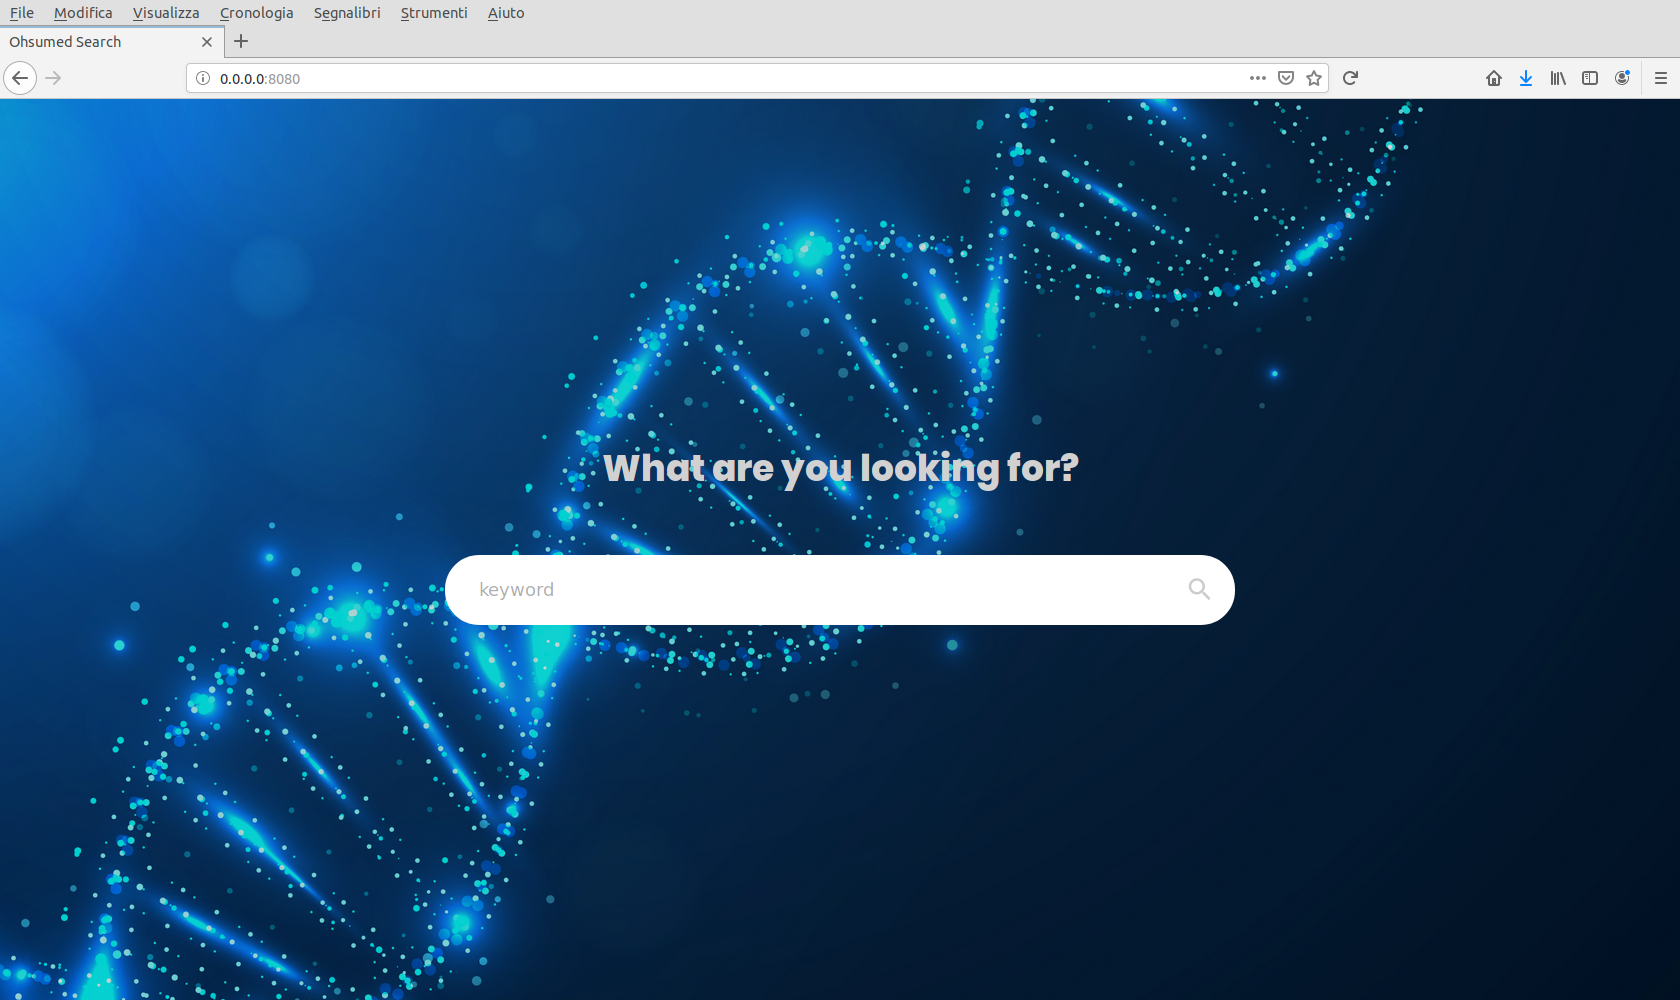
\includegraphics[width=1\linewidth]{index} }}%
    \caption{Pagina iniziale.}%
\end{figure}

Dopo aver effettuato il reperimento, l'utente viene indirizzato alle pagine contenenti
i link dei risultati.
Questi link poi rimandano alla pagina di \emph{PubMed}\footnote{\url{https://www.ncbi.nlm.nih.gov/pubmed/}} dove c'\`e l'articolo.

Se ne pu\`o vedere un esempio in Figura 3.

\begin{figure}%
    \centering
    {{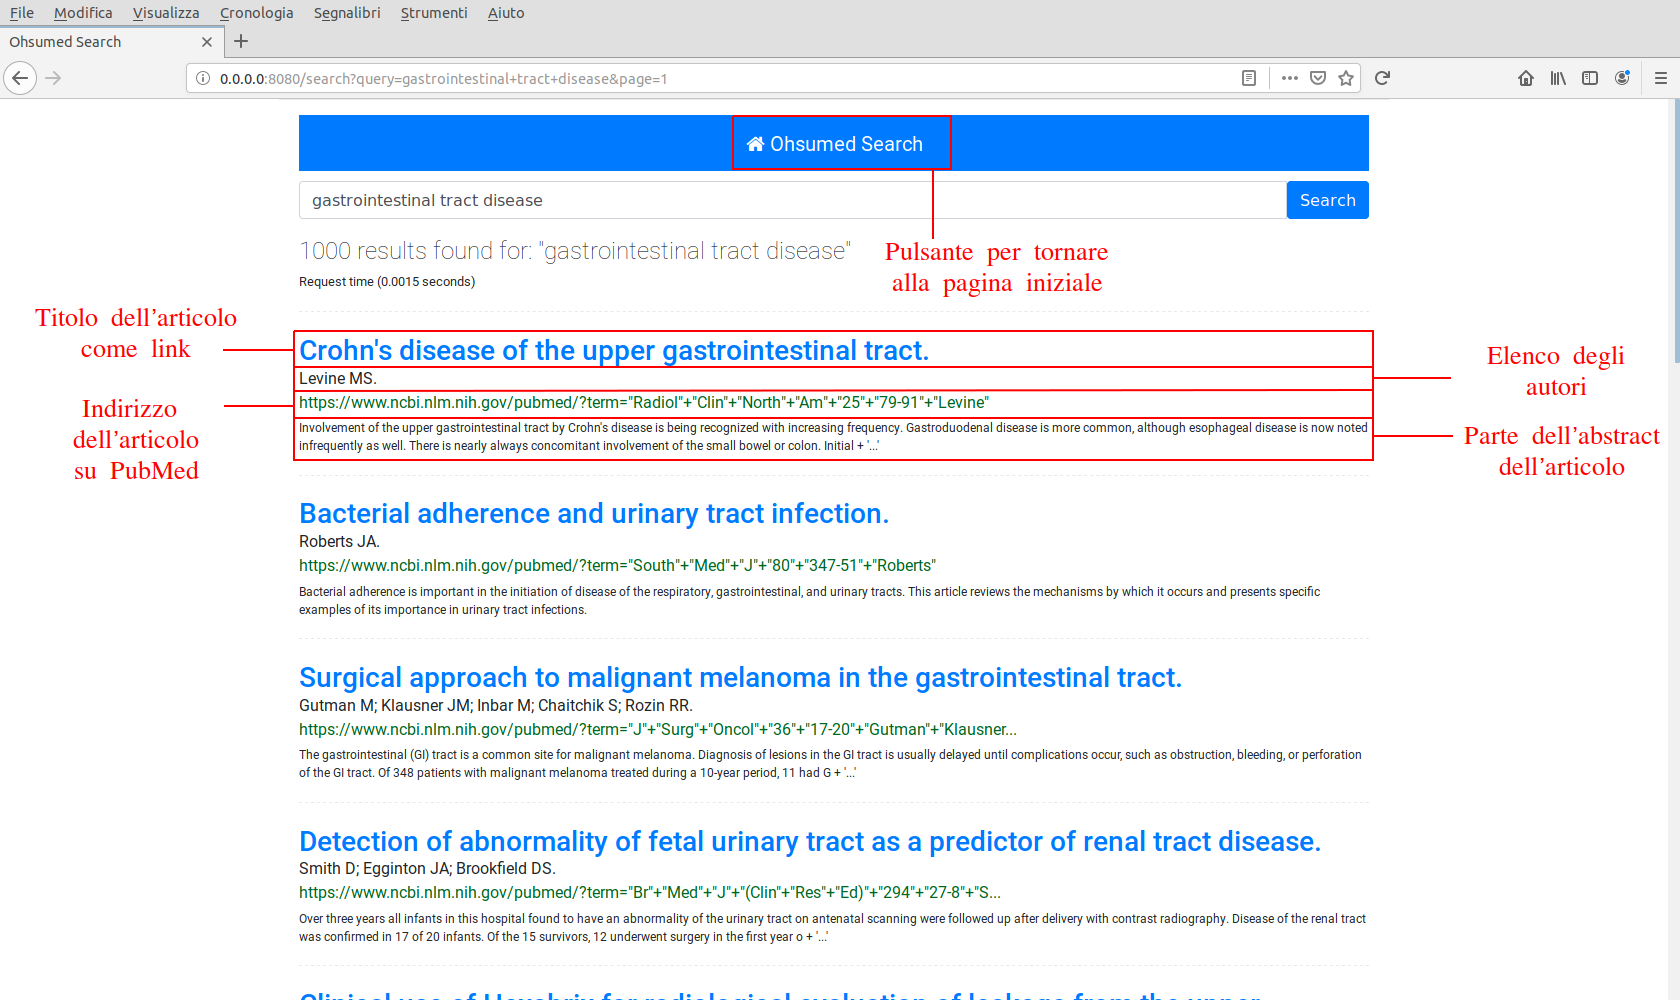
\includegraphics[width=1\linewidth]{risultati} }}%
    \caption{Pagina dei risultati.}%
\end{figure}

\`E risultato utile sfruttare un modulo legato a whoosh (paginate-whoosh\footnote{\url{https://pypi.org/project/paginate-whoosh/}})
che d\`a la possibilit\`a di ottenere facilmente la suddivisione dei risultati in pagine.

\begin{figure}%
    \centering
    {{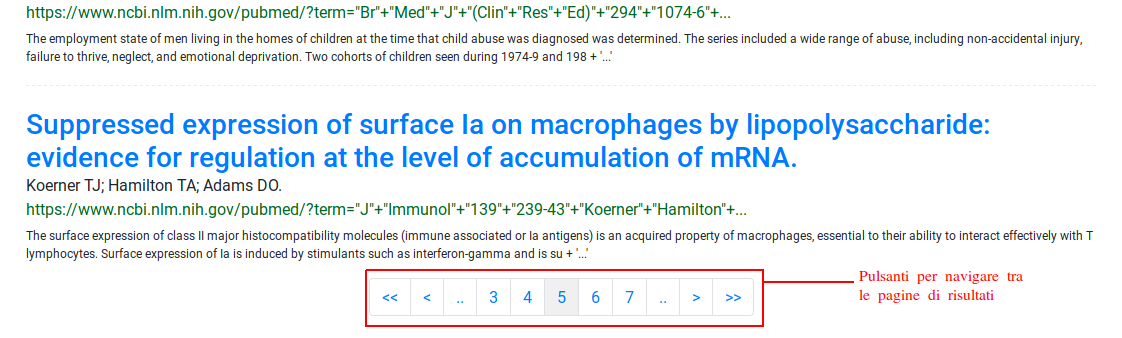
\includegraphics[width=1\linewidth]{pagination} }}%
    \caption{Pulsanti per navigare tra le pagine di risultati.}%
\end{figure}

Nel caso in cui non vengano trovati risultati si forniscono all'utente dei
suggerimenti per correggere eventualmente la query.

Per come \`e scritta la funzione di reperimento, non sarebbe difficile
implementare una funzionalit\`a di "ricerca avanzata" dando all'utente la possibilit\`a 
di cercare per autore o di scegliere l'operatore logico per collegare le parole
della query.

\section{Esperimenti e Risultati}
\label{sec:esperimenti}


Per gli esperimenti si \`e utilizzata parte della gi\`a citata collezione sperimentale chiamata OHSUMED\footnote{ \url{https://bit.ly/2wpOynZ}}.

Si tratta di una collezione di oltre 300'000 articoli provenienti dal database bibliografico MEDLINE pubblicati tra il 1987 ed il 1991; di questi documenti ne sono stati utilizzati 54'711.

I programmi utilizzati per effettuare indicizzazione e reperimento sono stati scritti in python(versione 2.7), sfruttando oggetti e funzioni del modulo whoosh\footnote{ \url{https://whoosh.readthedocs.io/en/latest/index.html}}.

Per la valutazione dei risultati ottenuti nei vari esperimenti si \`e invece utilizzato lo strumento standard trec\_eval\footnote{ \url{https://trec.nist.gov/trec\_eval/}}.
Questo programma permette di ottenere alcune misure della qualit\`a di un sistema di information retrieval se si conoscono i documenti rilevanti per le query sperimentali utilizzate.

Come misura da usare nel confronto tra risultati di diverse run si \`e scelta la Mean Average Precision(\textit{MAP})\cite{WBC_map} , quantit\`a calcolabile sia a livello di singola query che a livello complessivo su un insieme di query.
Inoltre, per verificare se i valori di \textit{MAP} ottenuti in run diverse si discostano in modo statisticamente significativo gli uni dagli altri si effettuano test di Wilcoxon\cite{WBC_Will} su coppie di risultati. \par

\subsection{Scelte iniziali}

Prima di iniziare gli esperimenti sono state fatte delle scelte riguardo certi aspetti dei metodi di reperimento che rimanessero costanti durante tutti gli esperimenti.
Queste scelte sono state fatte in seguito ad alcune run preliminari.

Come schema di pesatura, per la funzione di reperimento e ranking,  si \`e deciso di utilizzare il BM25F, descritto nella sezione precedente, anche perch\`e si pu\`o considereare "state-of-the-art" dal punto di vista dei modelli per information retrieval su documenti strutturati, e si \`e deciso di utilizzare l'operatore OR come operatore logico per raggruppare le parole delle query, ovvero si cercano documenti in cui \`e presente almeno una parola della query.

Sempre a seguito delle run preliminari si \`e deciso di utilizzare il campo "desc" delle query anzich\'e il campo "title" in quanto d\`a risultati migliori; inoltre, si \`e notato che in alcune query sperimentali sono presenti parole scritte in modo errato e che quindi non risultano presenti nell'indice.
Per questo dopo aver verificato, leggendo i documenti rilevanti per quelle query, quali fossero gli errori si \`e ritenuto opportuno effettuare una correzione al momento del reperimento.
A grandi linee, la correzione viene fatta su parole che non risultano presenti nell'indice cercando in quest'ultimo delle parole alternative che si discostano di al pi\`u una lettera dalla parola originale; queste parole vengono quindi aggiunte alla query di partenza e si procede con la ricerca.

Un'ultima scelta \`e stata fatta riguardo il numero massimo di documenti reperiti.
Si \`e optato per 100 documenti poich\'e un numero maggiore non porta grandi miglioramenti dal punto di vista del \textit{MAP}. \par

Affinch\'e Whoosh possa indicizzare una collezione di documenti, necessita la
specificazione di uno schema che include, per ogni possibile campo dei documenti della collezione, il nome del campo ed il tipo del campo.

Lo schema di base per la collezione qui utilizzata \`e il seguente:
\par

\begin{figure}
\vspace{-5mm}
\begin{lstlisting}
schema = Schema(docid      	= ID(stored=True),
		title      	= TEXT(stored=True),
		identifier	= ID(stored=True),
		terms 		= NGRAM(stored=True),
		authors		= NGRAM(stored=True),
		abstract 	= TEXT(stored=True),
		publication	= TEXT(stored=True),
		source 		= TEXT(stored=True))
\end{lstlisting}
      \caption{Schema necessario all'indicizzazione dei documenti. "stored=True" indica che il campo viene salvato ed \`e quindi successivamente accessibile. }
      \vspace{-10mm}
\end{figure}


\subsection{Baseline}
I valori di \textit{MAP} scelti come baseline sono quelli ottenuti effettuando ricerche su un indice con lo schema di base, riportato sopra, senza l'utilizzo di una lista di stopword e cercando in due campi dei documenti: "title" e "abstract".
Cercando su un campo ("title") o tre campi ("title", "abstract" e "terms") risulta solo in un peggioramento dei risultati.

Si possono vedere i risultati ottenuti usando la configurazione "baseline" riassunti in Tabella 1.
\par


\begin{table}
\vspace{-3mm}
\centering
\begin{tabular}{lll}
\hline
\textbf{ un campo }           & \textbf{ due campi }           & \textbf{ tre campi }            \\ \hline
 num\textit{q all 63 }       &  num\textit{q all 63 }       &  num\textit{q all 63 }        \\
 num\textit{ret all 6228 }  &  num\textit{ret all 6244 }  &  num\textit{ret all 6271 }   \\
 num\textit{rel all 670 }    &  num\textit{rel all 670 }    &  num\textit{rel all 670 }     \\
 num\textit{rel}ret all 349  &  num\textit{rel}ret all 419  &  num\textit{rel}ret all 367   \\
map all 0.2130               & map all \bf 0.2744               & map all 0.2155 \\ \hline
\end{tabular}

\caption{ Risultati trec\_eval complessivi per tutte le query, nessuna manipolazione del testo, numero risultati restituiti per
ogni query = 100, pesatura BM25F.}
\vspace{-7mm}
\end{table}

Come si nota dalla tabella il valore baseline di \textit{MAP} \`e 0.2744.
\par



\vskip 1.5in

\subsection{Esperimenti}

Gli esperimenti sono consistiti in tre prove in cui si \`e cambiato l'insieme di stopword usato nell'indicizzazione. In particolare ad ogni prova si \`e utilizzato un insieme di stopword con parole in pi\`u rispetto a quello delle prove precedenti.

Come con la baseline, per ciascuna prova si \`e effettuata la ricerca per uno, due e tre campi.

\subsubsection{Prima prova:}

Per la prima prova sono state utilizzate le stopword generali della lingua inglese. Queste comprendono termini come "the", "that", "is"; sono poi state aggiunte anche le lettere dell'alfabeto ed i numeri.

Come si vede in Tabella 2, non sembra si sia ottenuto un miglioramento significativo rispetto alla baseline. Il \textit{MAP} ottenuto utilizzando due campi "migliora" solo dello 0.0001.
\begin{table}
\vspace{-3mm}
\centering
\begin{tabular}{lll}
\hline
\textbf{ un campo }           & \textbf{ due campi }           & \textbf{ tre campi }            \\ \hline
 num\textit{q all 63 }       &  num\textit{q all 63 }       &  num\textit{q all 63 }        \\
 num\textit{ret all 6228 }  &  num\textit{ret all 6244 }  &  num\textit{ret all 6271 }   \\
 num\textit{rel all 670 }    &  num\textit{rel all 670 }    &  num\textit{rel all 670 }     \\
 num\textit{rel}ret all 350  &  num\textit{rel}ret all 418  &  num\textit{rel}ret all 367   \\
map all 0.2137               & map all \bf 0.2745               & map all 0.2152          \\ \hline
\end{tabular}

\caption{ Risultati trec\_eval, rimozione delle stopword generali, numero risultati restituiti per ogni query = 100, pesatura BM25F.}
\vspace{-7mm}
\end{table}

\subsubsection{Seconda prova:}

Nella seconda prova si \`e allora cercato di migliorare i risultati aggiungendo alle stopword generali, alcune parole che non sono normalmente considerate stopword ma che nel contesto medico, come nel caso della collezione OHSUMED, diventano tali.

Per questo abbiamo utilizzato un insieme di stopword denominate stopword\_cliniche che oltre ad avere le stopword generali ha anche parole come "medical", "condition" o "family"\footnote{ \url{https://github.com/kavgan/clinical-concepts/blob/master/clinical-stopwords.txt}}.

Con questa prova sono stati ottenuti risultati accettabili, infatti come si vede in Tabella 3, l'aumento del \textit{MAP} rispetto alla baseline \`e stato quasi dello 0.01:
\begin{table}
\vspace{-3mm}
\centering
\begin{tabular}{lll}
\hline
\textbf{ un campo }           & \textbf{ due campi }           & \textbf{ tre campi }            \\ \hline
 num\textit{q all 63 }       &  num\textit{q all 63 }       &  num\textit{q all 63 }        \\
 num\textit{ret all 6228 }  &  num\textit{ret all 6244 }  &  num\textit{ret all 6271 }   \\
 num\textit{rel all 670 }    &  num\textit{rel all 670 }    &  num\textit{rel all 670 }     \\
 num\textit{rel}ret all 350  &  num\textit{rel}ret all 419  &  num\textit{rel}ret all 376   \\
map all 0.2156               & map all \bf 0.2837               & map all 0.2166          \\ \hline
\end{tabular}

\caption{ Risultati trec\_eval, rimozione delle stopword cliniche, numero risultati restituiti per ogni query = 100, pesatura BM25F.}
\vspace{-7mm}
\end{table}


\subsubsection{Terza prova:}

Nell'ultima prova sono state aggiunte altre parole alla lista delle stopword. La scelta delle parole da aggiungere \`e stata fatta in due fasi principali.

Nella prima \`e stata ricavata la frequenza con cui le parole delle query appaiono nei rispettivi documenti rilevanti. Dopo di ci\`o le parole con frequenza prossima allo 0 sono state prese in considerazione come possibili stopword.

Nella seconda fase sono state prese le query che, basandosi sui risultati della seconda prova, hanno avuto un \textit{MAP} relativamente basso(inferiore a 0.2). Sono state quindi prese alcune parole di queste query come altre possibili stopword anche basandosi sulla loro frequenza nei documenti rilevanti.

Per alcune parole la scelta se includerle nell'insieme di stopword \`e stata resa difficile dal fatto che, essendo presenti in pi\`u di una query la loro rimozione poteva significare il miglioramento di un \textit{MAP} ed il peggioramento di un altro.

Per questo, prima di arrivare all'insieme finale sono stati fatti alcuni tentativi.

Come si pu\`o notare dalla Tabella 4 si ha un aumento del \textit{MAP} rispetto alla baseline decisamente superiore alle prove precedenti, con circa lo 0.075 in pi\`u.
\begin{table}
\vspace{-3mm}
\centering
\begin{tabular}{lll}
\hline
\textbf{ un campo }           & \textbf{ due campi }           & \textbf{ tre campi }            \\ \hline
 num\textit{q all 63 }       &  num\textit{q all 63 }       &  num\textit{q all 63 }        \\
 num\textit{ret all 5282 }  &  num\textit{ret all 5690 }  &  num\textit{ret all 5788 }   \\
 num\textit{rel all 670 }    &  num\textit{rel all 670 }    &  num\textit{rel all 670 }     \\
 num\textit{rel}ret all 386  &  num\textit{rel}ret all 463  &  num\textit{rel}ret all 435   \\
map all 0.2720               & map all \bf 0.3508               & map all 0.2813          \\ \hline
\end{tabular}

\caption{ Risultati trec\_eval, rimozione delle stopword cliniche migliorate, numero risultati restituiti per ogni query = 100, pesatura BM25F.}
\vspace{-7mm}
\end{table}

La Figura 6 riassume i risultati delle tre prove e si pu\`o notare un netto miglioramento utilizzando le stopword migliorate.


\begin{figure}%
    \centering
    {{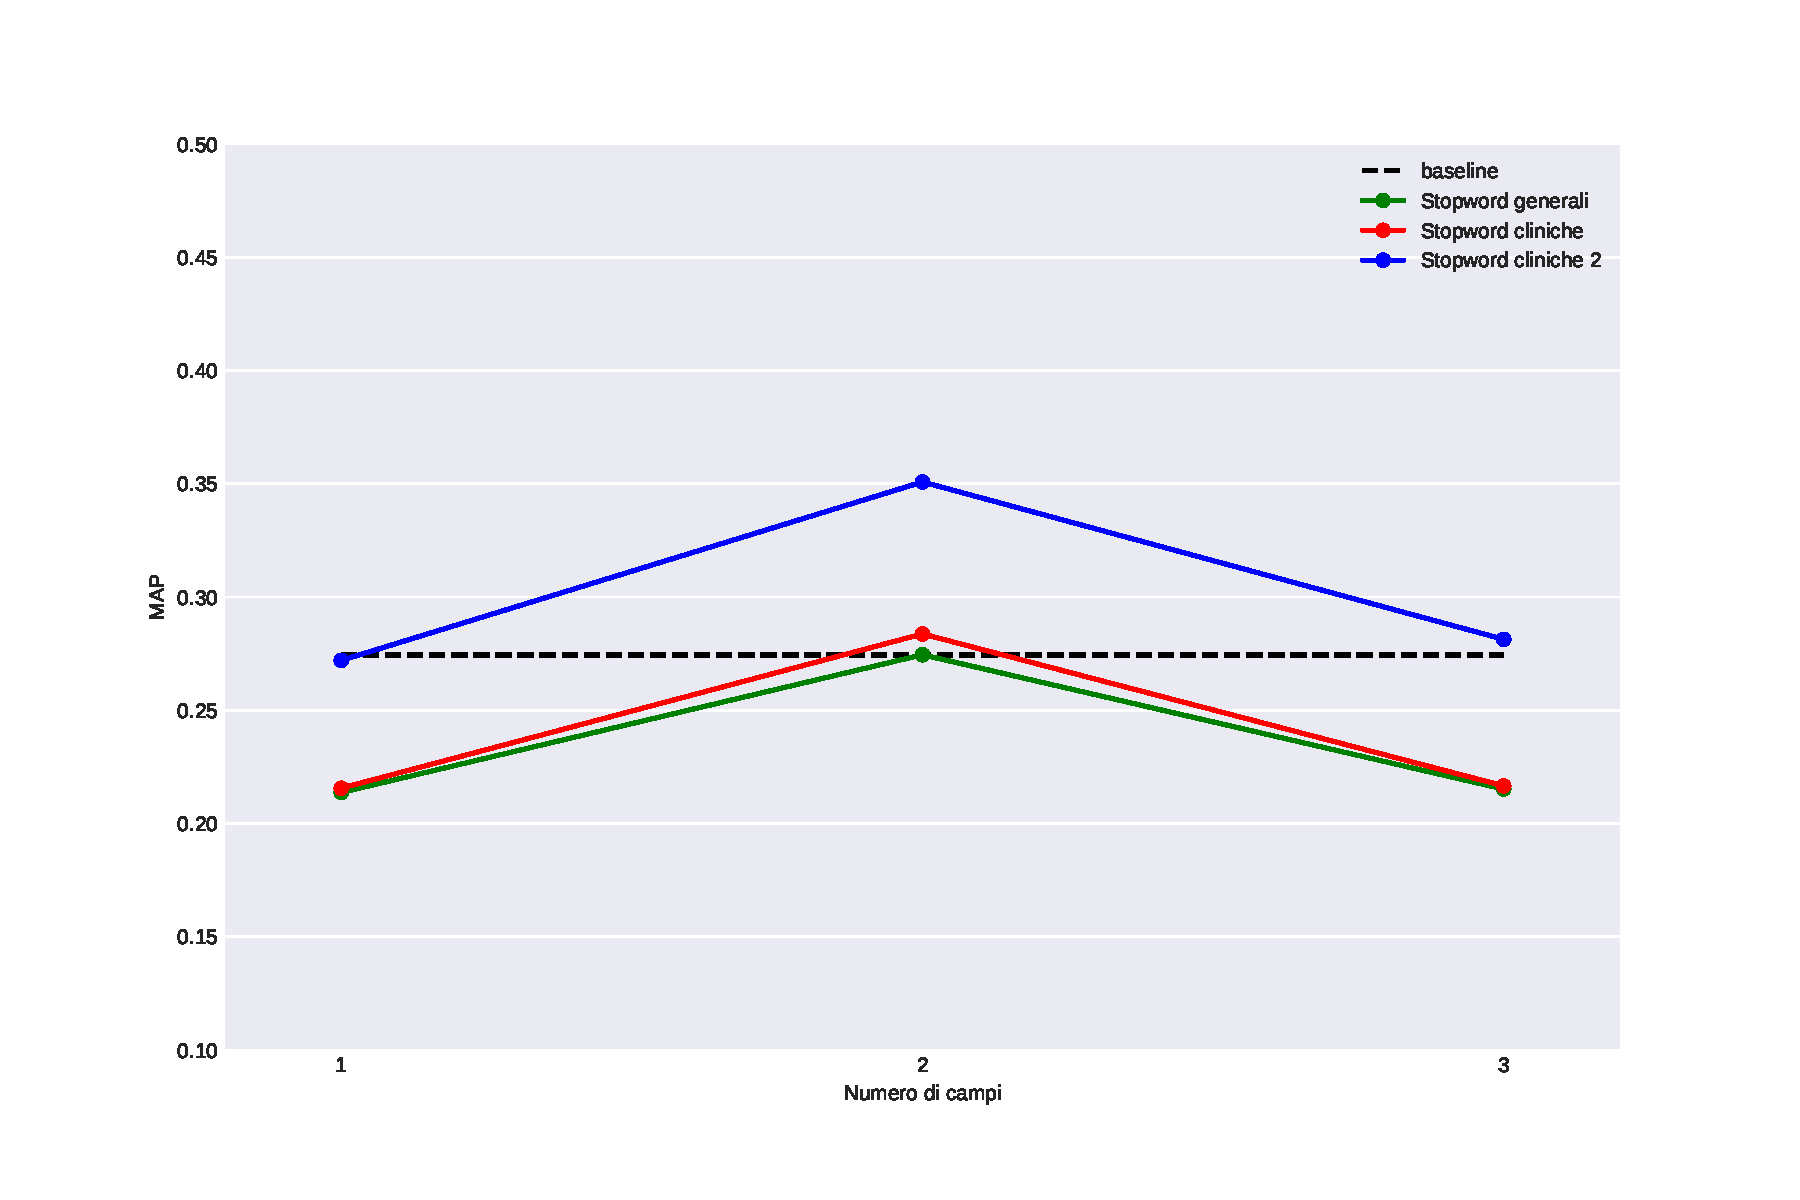
\includegraphics[width=0.8\linewidth]{maps} }}%
    \caption{Variazione del \textit{MAP} cambiando il numero di campi per i tre insiemi di stopword, la linea orizzontale indica la baseline di 0.2744.}%
    \vspace{-10mm}
\end{figure}


\subsection{Test di significativit\`a :}
\vspace{-5mm}
Per avere conferma che le differenze tra i \textit{MAP} ottenuti nelle varie prove e nella baseline
siano significativamente diversi si \`e ritenuto opportuno effettuare dei test.
Tra i test che si utilizzano comunemente a questo scopo si \`e scelto di utilizzare il
test di Wilcoxon che a differenza dell'alternativo t-test risulta avere pi\`u
potenza statistica in caso di non normalit\`a dei dati.

I test sono stati fatti tra i \textit{MAP} delle prove utilizzando due campi in quanto hanno
dato generalmente risultati migliori.

L'ipotesi alternativa \`e unilaterale ed equivale a dire che, tra le due prove
confrontate, la seconda prova ha \textit{MAP} maggiore della prima.
Per contro l'ipotesi nulla \`e che la prima prova ha \textit{MAP} maggiore o uguale alla seconda.

\begin{table}
\centering
\begin{tabular}{lll}
\hline
\textbf{ Prove a confronto }  & \textbf{ statistica test }  & \textbf{ p-value }            \\ \hline
 BASELINE contro STOP1  &  582      &  0.0393       \\
 BASELINE contro STOP2  &  551.5    &  0.0092       \\
 STOP1 contro STOP2     &  549.5    &  0.0056       \\
 BASELINE contro STOP3  &  276.0    &  $1.2749\mathrm{e}{-6}$   \\
 STOP1 contro STOP3     &  291.0    &  $1.2936\mathrm{e}{-6}$   \\
 STOP2 contro STOP3     &  290.0    &  $3.5437\mathrm{e}{-6}$   \\ \hline
\end{tabular}

\caption{ Statistiche test e livelli di significativit\`a osservati per i test sulla differenza dei \textit{MAP}.
STOP1 indica le stopword generali, STOP2 indica le stopword cliniche e STOP3 indica le stopword cliniche migliorate.}
\vspace{-5mm}
\end{table}

Come si vede in Tabella 5 i miglioramenti portati dalle stopword delle prime due prove hanno p-value che permettono di rifiutare l'ipotesi nulla solo in caso si prenda come soglia il livello di significativit\`a dello 0.05.
Invece, con la terza prova il p-value risulta molto pi\`u basso portando a rifiutare l'ipotesi nulla in maniera pi\`u convincente.


\section{Considerazioni finali}
%\section{Conclusione}
\vspace{-5mm}
Come si \`e visto dai risultati delle prove, l'utilizzo di stopword inerenti al contesto
della collezione, porta a reperire pi\`u documenti rilevanti nelle prime posizioni.
Bisogna, per\`o, tenere in considerazione che nella terza prova, quella che ha dato
i risultati migliori, l'insieme delle stopword creato \`e strettamente legato alle
query sperimentali. Per questo c'\`e la possibilit\`a che i risultati ottenuti con query diverse
siano peggiori.

\vskip 1.5in

\begin{thebibliography}{8}

\bibitem{WBC}
W. Bruce Croft and Donald Metzler and Trevor Strohman. Search Engines: Information Retrieval in Practice. Addison Wesley, (2009), pp. 250-252

\bibitem{WBC_stopword}
W. Bruce Croft and Donald Metzler and Trevor Strohman. Search Engines: Information Retrieval in Practice. Addison Wesley, (2009), pp. 90-91

\bibitem{WBC_map}
W. Bruce Croft and Donald Metzler and Trevor Strohman. Search Engines: Information Retrieval in Practice. Addison Wesley, (2009), pp. 313

\bibitem{WBC_Will}
W. Bruce Croft and Donald Metzler and Trevor Strohman. Search Engines: Information Retrieval in Practice. Addison Wesley, (2009), pp. 325-330

\bibitem{WBC_ii}
W. Bruce Croft and Donald Metzler and Trevor Strohman. Search Engines: Information Retrieval in Practice. Addison Wesley, (2009), pp. 129-130

\bibitem{PRP}
S.E. Robertson, (1997) "THE PROBABILITY RANKING PRINCIPLE IN IR", Journal of Documentation, Vol. 33 Issue: 4, pp.294-304, https://doi.org/10.1108/eb026647

\end{thebibliography}

\begin{figure}[h!]
  \subfigure[Alessandro Stefani]{
    
\includegraphics[width=35mm,height=35mm]{aleste}}
  \subfigure[Caterina Buranelli]{
    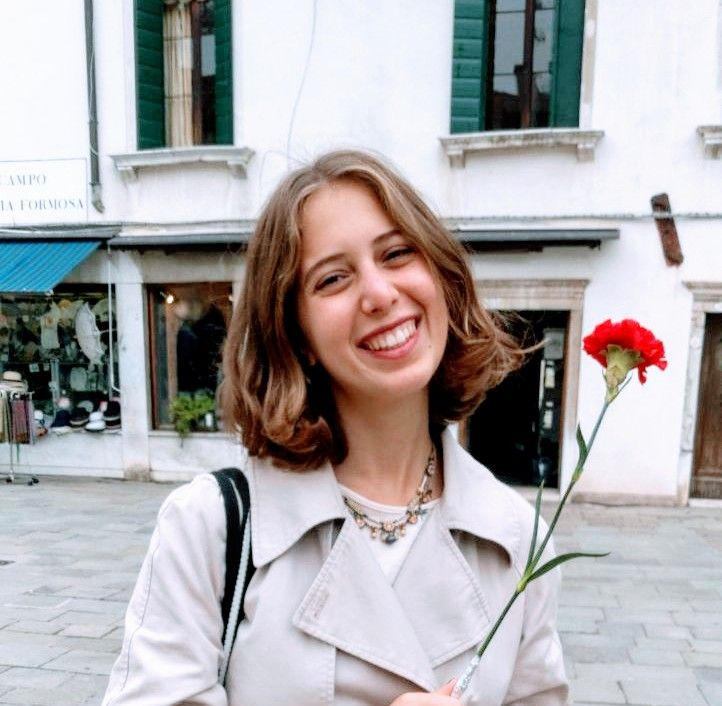
\includegraphics[width=35mm,height=35mm]{caterina}}
  \subfigure[Cristi Gutu]{
    
\includegraphics[width=35mm,height=35mm]{cristi}}
\end{figure}

\end{document}
